\section{译者补充:辐射度学与光度学}\label{sec:译者补充:辐射度学与光度学}

\begin{remark}
      本节内容不是原书内容,而是译者根据有关资料\citep{978-7-5640-0658-7,
            wiki:solidangle,GB3102.6-93,enwiki:1052681830,
            wiki:candela,Hoffmann2015}补充的,请酌情参考和斧正。
\end{remark}

\subsection{辐射度量}\label{sub:辐射度量}
立体角表示一个物体对特定点的三维空间角度,是平面角在三维空间中的类比。
它描述在某一点观测到的物体大小尺度。
例如对于一特定观察点,一个在该点附近的小物体
可能和一个远处的大物体有着相同的立体角。
\begin{definition}
      锥体的\keyindex{立体角}{solid angle}{}大小定义为:
      以锥体的顶点为球心作球面,该锥体在球表面截取的面积与球半径平方之比。
\end{definition}
立体角的单位为\keyindex{球面度}{steradian}{}(sr),是无量纲的导出单位。

\begin{figure}[htbp]
      \centering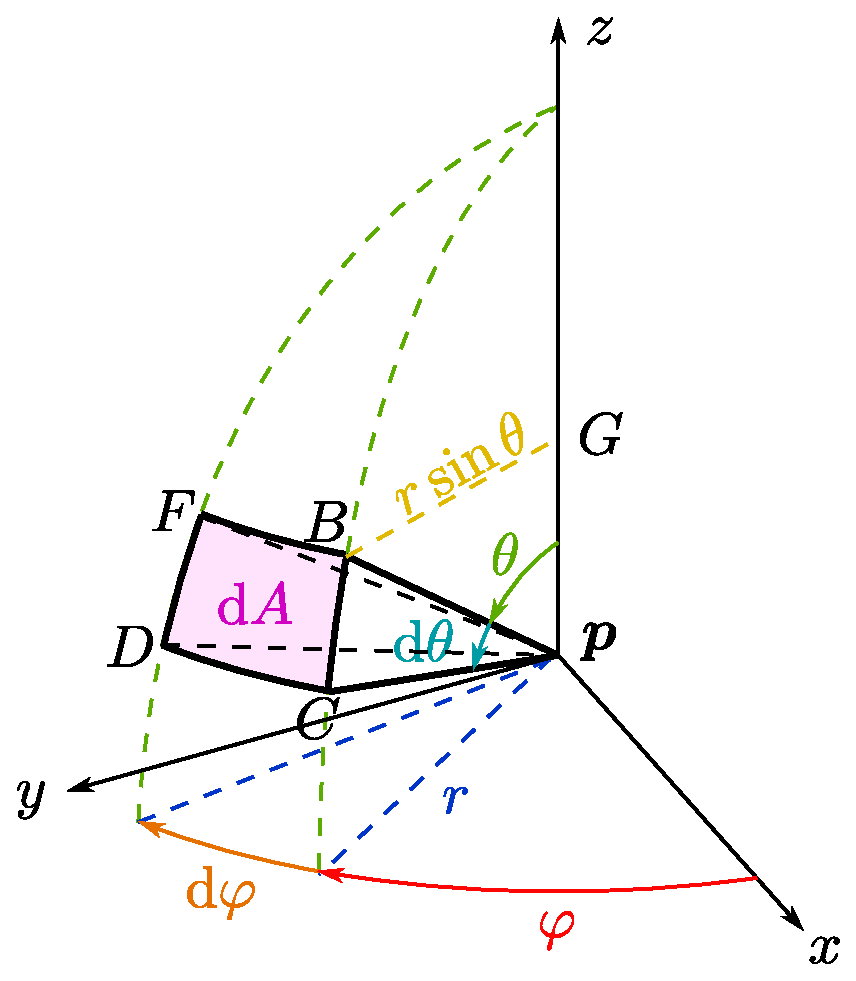
\includegraphics[width=0.4\linewidth]{chap05/ex-solidangle.eps}
      \caption{立体角的定义。}
      \label{fig:5.ex01}
\end{figure}

立体角常用字母$\varOmega$表示。\reffig{5.ex01}展示了一种简单的情形。
以$\bm p$为顶点的微分锥体${\bm p}-BCDF$在同样以$\bm p$为球心且半径为$r$的球面上截取下面元$BCDF$。
建立以$\bm p$为原点的球坐标系,则弧线$\wideparen{BC}$的\keyindex{方位角}{azimuth angle}{}
(在$xy$平面上的投影与原点连线和$x$正半轴所成角)为$\varphi$,
$\wideparen{DF}$方位角为$\varphi+\mathrm{d}\varphi$;
弧线$\wideparen{BF}$的\keyindex{天顶角}{zenith angle}{}(与原点连线和$z$正半轴所成角)为$\theta$,
$\wideparen{CD}$的天顶角为$\theta+\mathrm{d}\theta$。
因此点$B$到其在$z$轴投影点$G$的距离为$r\sin\theta$,
$\wideparen{BF}$的弧长为$r\sin\theta\mathrm{d}\varphi$;
同时$\wideparen{BC}$的弧长为$r\mathrm{d}\theta$。
将面元$BCDF$视作矩形,可求得其微分面积为
\begin{align}
      \mathrm{d}A=r\sin\theta\mathrm{d}\varphi\cdot r\mathrm{d}\theta\, .
\end{align}
依据定义,则相应的立体角元为
\begin{align}
      \mathrm{d}\varOmega=\frac{\mathrm{d}A}{r^2}=\sin\theta\mathrm{d}\theta\mathrm{d}\varphi\, .
\end{align}
对立体角元做曲面积分则可得立体角
\begin{align}
      \varOmega=\iint\limits_S \mathrm{d}\varOmega=\iint\limits_S \sin\theta\mathrm{d}\theta\mathrm{d}\varphi\, .
\end{align}

\begin{corollary}
      封闭曲面对于其内任意一点的立体角均为$4\pi$sr。
\end{corollary}

在连续意义下,我们定义以下辐射度量。

\begin{definition}
      \keyindex{辐射能}{radiant energy}{}指以电磁波形式发射、传播或接收的能量。
\end{definition}
辐射能常用$Q$表示,单位为\keyindex{焦耳}{joule}{}(焦,J)。

\begin{definition}
      \keyindex{辐射能通量}{radiant energy flux}{},
      也称\keyindex{辐射功率}{radiant power}{},
      指电磁辐射通过某一面积发射、传播或接收的功率。
\end{definition}
辐通量常用$\varPhi$表示,单位为\keyindex{瓦特}{watt}{}(瓦,W)。
它描述单位时间内的辐射能:
\begin{align}
      \varPhi=\frac{\mathrm{d}Q}{\mathrm{d}t}\, ,
\end{align}
其中$t$表示时间。

\begin{definition}
      \keyindex{辐射照度}{irradiance}{}指照射到表面一点处的
      单位面元上的辐射能通量。
\end{definition}
\begin{definition}
      \keyindex{辐射出射度}{radiant exitance}{}指离开表面一点处的
      单位面元上的辐射能通量。
\end{definition}
辐射照度常用$E$表示,辐射出射度常用$M$表示,单位均为$\text{W}/\text{m}^2$。
它们定义中面元所对应的立体角是辐射的整个半球空间,与辐通量的关系为
\begin{align}
      E(\text{或}M)=\frac{\mathrm{d}\varPhi}{\mathrm{d}A}\, ,
\end{align}
其中$A$为表面面积。

\begin{definition}
      \keyindex{辐射强度}{radiant intensity}{}指
      在给定方向的单位立体角元内离开点辐射源(或辐射源面元)的辐射通量。
\end{definition}
辐射强度常用$I$表示,单位为$\text{W}/\text{sr}$。
它一般适合于描述(近似)点光源的辐射方向特性,
与辐射通量和立体角的关系为
\begin{align}
      I=\frac{\mathrm{d}\varPhi}{\mathrm{d}\varOmega}\, .
\end{align}

\begin{definition}
      \keyindex{辐射亮度}{radiance}{}指
      表面一点在垂直于给定方向的单位面元上于该方向的辐射强度。
\end{definition}
辐射亮度常用$L$表示,单位为W$/$(sr$\cdot$m$^2$)。
它与其他辐射度量的关系为
\begin{align}\label{eq:5.ex-radiance}
      L=\frac{\mathrm{d}I}{\cos\theta\mathrm{d}A}=\frac{\mathrm{d}^2\varPhi}{\cos\theta\mathrm{d}A\mathrm{d}\varOmega}=\frac{\mathrm{d}E}{\cos\theta\mathrm{d}\varOmega}\, ,
\end{align}
其中$\theta$是曲面法线与给定方向的夹角。

\reffig{5.ex02}展示了辐射度量之间的微分关系。
\begin{figure}[htbp]
      \centering
      \begin{picture}(370,50)
            \put(0,0){辐射能$Q$}
            \put(45,3){\vector(1,0){40}}
            \put(50,6){时间$t$}
            \put(90,0){辐射通量$\varPhi$}
            \put(150,3){\vector(1,0){50}}
            \put(152,6){立体角$\varOmega$}
            \put(205,0){辐射强度$I$}
            \put(260,3){\vector(1,0){50}}
            \put(262,6){投影面积}
            \put(315,0){辐射亮度$L$}
            \put(120,12){\line(0,1){25}}
            \put(120,37){\vector(1,0){80}}
            \put(152,40){面积$A$}
            \put(205,35){辐射照度$E$}
            \put(260,37){\line(1,0){80}}
            \put(340,37){\vector(0,-1){25}}
            \put(262,40){余弦加权立体角}
      \end{picture}
      \caption{辐射度量的微分关系。}
      \label{fig:5.ex02}
\end{figure}

\subsection{光度学}\label{sub:光度学}
光度量是光辐射能为平均人眼接收所引起的视觉刺激大小的度量。
光度量和辐射度量的定义是一一对应的,所用字母相同,
作区分时两者常分别添加下标v和e。
它们都可以用来定量描述辐射的大小。
辐射度量是辐射能本身的客观度量,是纯粹的物理量;
而光度量则还考虑了生理学、心理学等因素。

\keyindex{发光强度}{luminous intensity}{}与辐射强度对应,
单位为坎德拉。
\begin{definition}
      频率为$540\times10^{12}\text{Hz}$的单色辐射光源
      在给定方向上辐射强度为$\displaystyle\frac{1}{683}$W$/$sr时,
      其发光强度为1\keyindex{坎德拉}{candela}{}(cd)。
\end{definition}
坎德拉是国际单位制七个基本单位之一。
一只普通蜡烛的发光强度约为1cd。

\keyindex{光通量}{luminous flux}{}与辐射通量对应,
单位为\keyindex{流明}{lumen}{}(lm),1lm$=$1cd$\cdot$sr。

注意到发光强度与光的频率有关,这是人眼视觉特性决定的。
例如在辐射功率一定时,人眼会感觉黄绿光比红光和蓝光看起来更明亮,即发光强度不同。


